\documentclass[]{article}
\usepackage[T1]{fontenc}
\usepackage{lmodern}
\usepackage{amssymb,amsmath}
\usepackage{ifxetex,ifluatex}
\usepackage{fixltx2e} % provides \textsubscript
% Set line spacing
% use upquote if available, for straight quotes in verbatim environments
\IfFileExists{upquote.sty}{\usepackage{upquote}}{}
\ifnum 0\ifxetex 1\fi\ifluatex 1\fi=0 % if pdftex
  \usepackage[utf8]{inputenc}
\else % if luatex or xelatex
  \ifxetex
    \usepackage{mathspec}
    \usepackage{xltxtra,xunicode}
  \else
    \usepackage{fontspec}
  \fi
  \defaultfontfeatures{Mapping=tex-text,Scale=MatchLowercase}
  \newcommand{\euro}{€}
\fi
% use microtype if available
\IfFileExists{microtype.sty}{\usepackage{microtype}}{}
\usepackage[margin=1in]{geometry}
\usepackage{graphicx}
% Redefine \includegraphics so that, unless explicit options are
% given, the image width will not exceed the width of the page.
% Images get their normal width if they fit onto the page, but
% are scaled down if they would overflow the margins.
\makeatletter
\def\ScaleIfNeeded{%
  \ifdim\Gin@nat@width>\linewidth
    \linewidth
  \else
    \Gin@nat@width
  \fi
}
\makeatother
\let\Oldincludegraphics\includegraphics
{%
 \catcode`\@=11\relax%
 \gdef\includegraphics{\@ifnextchar[{\Oldincludegraphics}{\Oldincludegraphics[width=\ScaleIfNeeded]}}%
}%
\ifxetex
  \usepackage[setpagesize=false, % page size defined by xetex
              unicode=false, % unicode breaks when used with xetex
              xetex]{hyperref}
\else
  \usepackage[unicode=true]{hyperref}
\fi
\hypersetup{breaklinks=true,
            bookmarks=true,
            pdfauthor={bdanalytics},
            pdftitle={Dutch Environmental Permit Application Process: CoSeLoG},
            colorlinks=true,
            citecolor=blue,
            urlcolor=blue,
            linkcolor=magenta,
            pdfborder={0 0 0}}
\urlstyle{same}  % don't use monospace font for urls
\setlength{\parindent}{0pt}
\setlength{\parskip}{6pt plus 2pt minus 1pt}
\setlength{\emergencystretch}{3em}  % prevent overfull lines
\setcounter{secnumdepth}{5}

%%% Change title format to be more compact
\usepackage{titling}
\setlength{\droptitle}{-2em}
  \title{Dutch Environmental Permit Application Process: CoSeLoG}
  \pretitle{\vspace{\droptitle}\centering\huge}
  \posttitle{\par}
  \author{bdanalytics}
  \preauthor{\centering\large\emph}
  \postauthor{\par}
  \date{}
  \predate{}\postdate{}




\begin{document}

\maketitle


{
\hypersetup{linkcolor=black}
\setcounter{tocdepth}{2}
\tableofcontents
}
\textbf{Date: (Wed) Dec 10, 2014}

Data: Originates from the CoSeLoG project executed under NWO project
number 638.001.211. Within the CoSeLoG project the (dis)similarities
between several processes of different municipalities in the Netherlands
has been investigated. This event log contains the records of the
execution of the receiving phase of the building permit application
process in an anonymous municipality.

Source:
\url{http://data.3tu.nl/repository/uuid:a07386a5-7be3-4367-9535-70bc9e77dbe6}

Time period: 2010-10-02 to 2012-01-23

\subsubsection{Synopsis:}\label{synopsis}

\paragraph{Potential next steps
include:}\label{potential-next-steps-include}

\subsubsection{Template:}\label{template}

\textbf{Approach I used}:\\Describe exactly what you did (e.g.~which
plug-ins did you use, which settings did you change), in such a way that
others can easily reproduce your results. You only need to describe
where/if you deviated from the provided instructions.

\textbf{What I saw}:\\Briefly describe the resulting analysis screen
(also include this as a screenshot, see explanation below), explain what
we see, without including observations or conclusions.

\textbf{My analysis}:\\What can you conclude from the analysis result?
How do you interpret the result? What is the answer to the question?

\subsubsection{Step 01: import event log in
Disco}\label{step-01-import-event-log-in-disco}

\textbf{Approach I used}:\\1. Import the event log into Disco.\\2.
Switch to ``Statistics'' tab / view\\3. Click on ``Overview'' button in
the left pane under ``Statistics views''\\4. Click on ``Events per
case'' button to the left of the graph

\textbf{What I saw}:

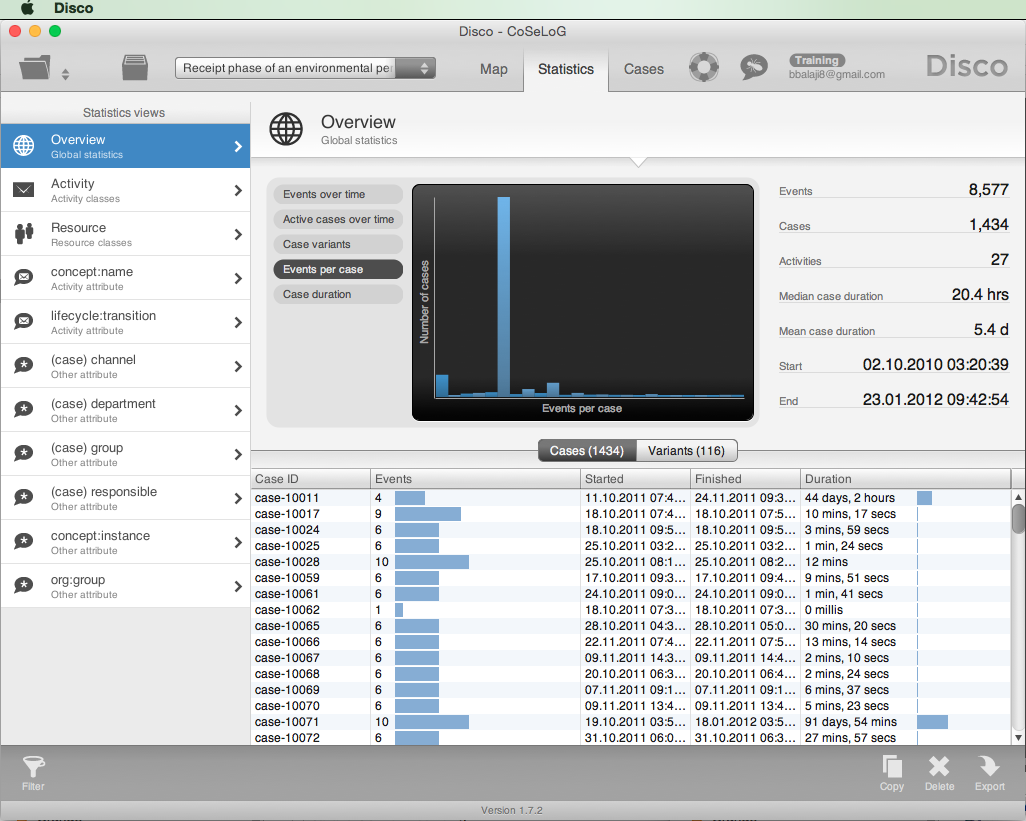
\includegraphics{CoSeLoG_Step_01_Q_01.png}

The graph pane displays a histogram (Number of cases) of Events per case
in this event log. The event log contains 8,577 events in 1,434 cases
with 27 activities.

\textbf{My analysis}:\\There are 6 events on average per case. This
information can be gathered by hovering the mouse on the tallest bar.

By clicking on ``Variants'' button on top of the table, we can see that
there are only 116 variants amongst the 1,434 cases.

The main observation from the `Events over time' graph is that the
maximum number of events (33) occured on May 2, 2011 across cases.

\subsubsection{Step 02: inspect process map in
Disco}\label{step-02-inspect-process-map-in-disco}

\textbf{Approach I used}:\\1. Click on ``Map'' tab in the window
header.\\2. Set ``Activities'' slider to 0\% \& ``Paths'' slider to 50\%
to make the process map fit on one screen and still be readable.

\textbf{What I saw}:

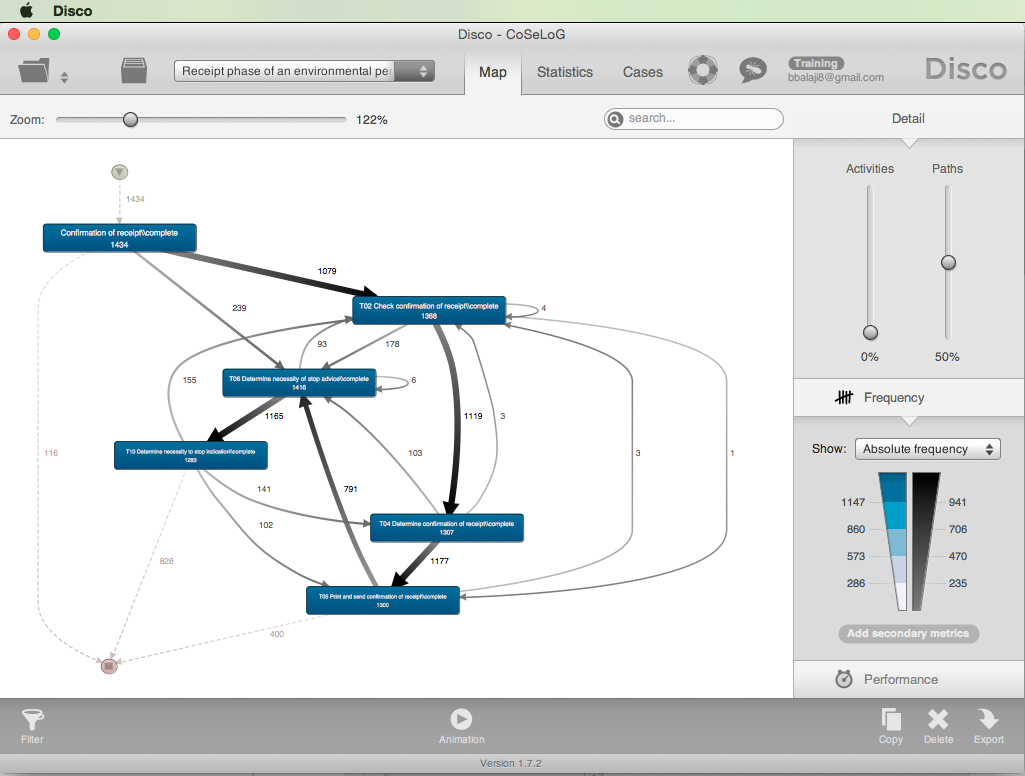
\includegraphics{CoSeLoG_Step_02.png}

\textbf{My analysis}:

The 6 most frequent activities between the initiation and termination of
cases in the process map include:\\A. Confirmation of receipt\\B. T02
Check confirmation of receipt\\C. T04 Determine confirmation of
receipt\\D. T05 Print and send confirmation of receipt E. T06 Determine
necessity of stop advice\\F. T10 Determine necessity to stop indication

The most frequent activity paths traced by the cases include (this is
supposed to display as a table, but doesn't work properly) :

\begin{verbatim}
                                    Activity Path | # of Cases  
\end{verbatim}

----------------------------------------------------- \textbar{}
-----------\\ Start -\textgreater{} TA -\textgreater{} End \textbar{}
116\\ Start -\textgreater{} TA -\textgreater{} T02 -\textgreater{} T04
-\textgreater{} T05 -\textgreater{} End \textbar{} 400\\Start
-\textgreater{} TA -\textgreater{} T02 -\textgreater{} T04
-\textgreater{} T05 -\textgreater{} T06 -\textgreater{} T10
-\textgreater{} End \textbar{} 828\\ \textbar{}\\ Total cases displayed
in this map \textbar{} 1,344\\ Total cases \textbar{} 1,434\\ \% cases
displayed in this map \textbar{} 94\%

Do not understand why if `` Confirmation of receipt'' is complete, there
is a need for ``T02 Check confirmation of receipt''. Additionally, there
are 4 activities (TA, T02, T04 \& T05) regarding confirmation of
receipts. Maybe these activities are not named appropriately ? and/or We
need to understand the intermediate activities (e.g.~T01, T03) to get a
better understanding ?

\subsubsection{Step 03: inspect process performance in
Disco}\label{step-03-inspect-process-performance-in-disco}

\textbf{Approach I used}:\\1. Click on ``Performance'' bar / button in
the ``Detail'' pane (right above the ``Copy'' / ``Delete'' / ``Export''
icons). 2. Select ``Total Duration'' in the ``Performance'' pane to
display. 3. Select ``Case frequency'' as the secondary metric in the
``Performance'' pane to ensure that we don't use outliers (e.g.~low case
frequency) to make broad conclusions about the process. 4. Cycle through
different metrics in the button next to ``Show:'' in the Performance
pane.

\textbf{What I saw}:

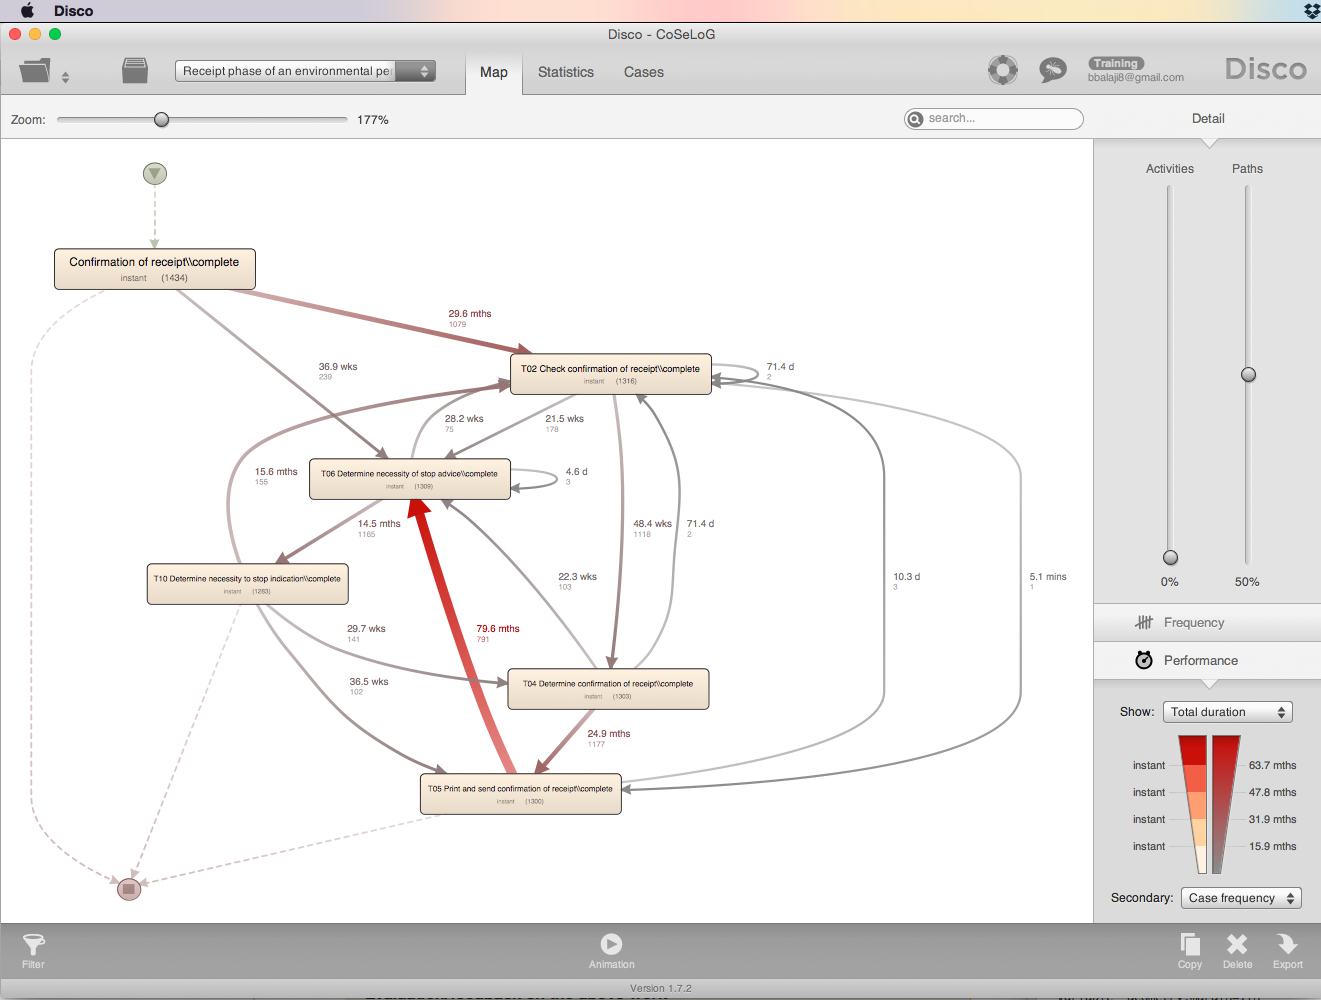
\includegraphics{CoSeLoG_Step_03.png}

The color \& thickness of the arcs are based on the distribution of the
selected primary performance metric. Additionally, if an arc is clicked,
a statistics window is dsiplayed for that arc.

\textbf{My analysis}:\\\emph{Total Duration}: The arc from T05 to T06
takes 79.6 months for 791 cases (31\% of total duration of all cases
which is 258.12 months: mean of 5.4 days per case X 1,434 cases / 30
elapsed days per month). The next bottleneck seems to be TA
-\textgreater{} T02 which is 29.6 months for 1,079 cases.

Analysis of other metrics (median, mean \& max duration) highlighted
arcs with very low case frequency.

\subsubsection{Step nn: step title}\label{step-nn-step-title}

\textbf{Approach I used}:

\textbf{What I saw}:

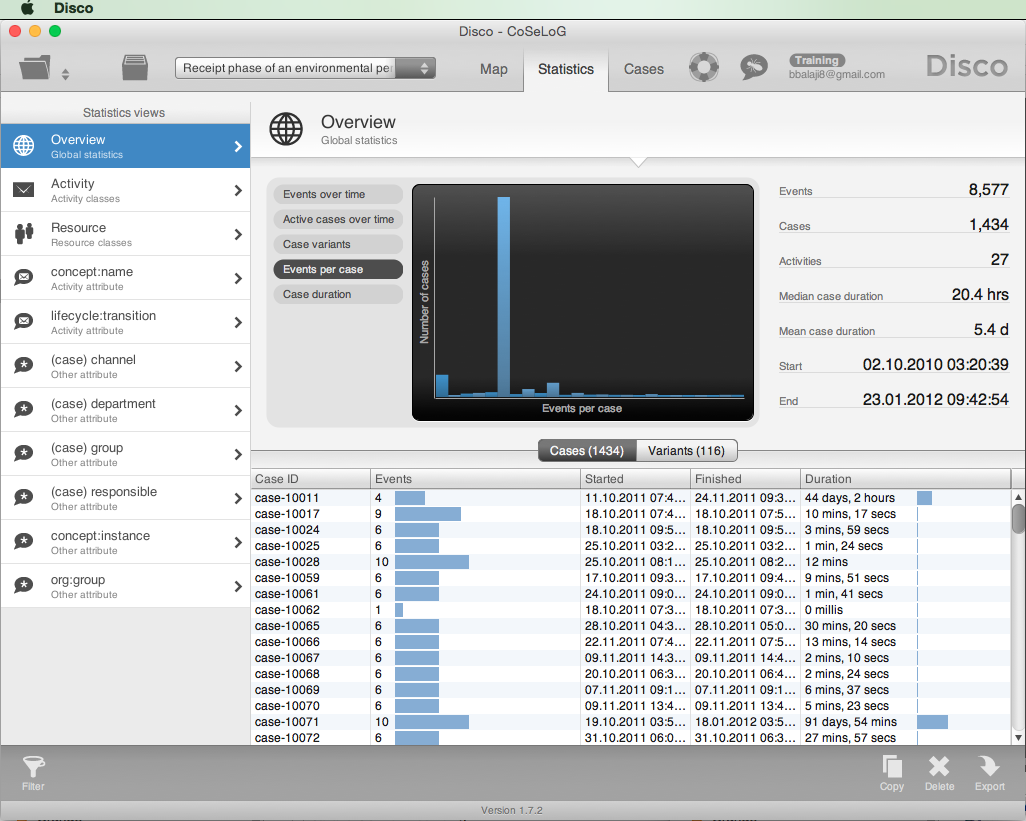
\includegraphics{dummy.png}

\textbf{My analysis}:

\end{document}
